\documentclass[paper=a4,twoside,abstract=on,cleardoublepage=empty,numbers=noenddot,toc=bib,12pt,appendixprefix=true]{scrreprt}

\usepackage[T1]{fontenc}
\usepackage[utf8]{inputenc}
\usepackage{lmodern}
\usepackage[scaled]{beramono}
\usepackage[ngerman,english]{babel}
\usepackage{todonotes}
\usepackage[style=numeric]{biblatex}
    \addbibresource{bibliography.bib}

%\setcitestyle{super,square}

\usepackage{blindtext}
\usepackage{multicol}
\usepackage{graphicx}
    \graphicspath{ {images/} }
\usepackage{pgfplots, pgfplotstable}
    \pgfplotsset{compat=1.8}
    \usepgfplotslibrary{statistics}
    \pgfplotsset{
        boxplotcompare style/.style={
            boxplot/draw direction=x,
            % width of boxes:
            boxplot/box extend=0.3,
            % visualize the median as a circle:
            boxplot/draw/median/.code={%
                \draw[fill=white]
                (boxplot cs:\pgfplotsboxplotvalue{median}) circle (3pt)
                ;
            },
        },
        rshift/.style={
            yshift=+\pgfkeysvalueof{/pgfplots/rshift scale},
            legend image post style={yshift=-\pgfkeysvalueof{/pgfplots/rshift scale}},
            solid,
            fill=gray,
            thick,
        },
        lshift/.style={
            yshift=-\pgfkeysvalueof{/pgfplots/lshift scale},
            legend image post style={yshift=\pgfkeysvalueof{/pgfplots/lshift scale}},
            solid,
            fill=white,
            thick,
        },
        rshift scale/.initial=1.2em,
        lshift scale/.initial=1.2em,
    }

\usetikzlibrary{patterns}
    \makeatletter
    \newcommand\resetstackedplots{
        \makeatletter
        \pgfplots@stacked@isfirstplottrue
        \makeatother
        \addplot [forget plot,draw=none] coordinates{(1,0) (2,0) (3,0) (4,0) (5,0) (6,0) (7,0) (8,0) (9,0) (10,0) (11,0)};
    }
    \makeatother

\usepackage{soul}
    \sethlcolor{darkgray}
    \newcommand{\invert}[1]{\textcolor{white}{\hl{#1}}}
    \newcommand{\cursor}{\invert{ }}
    \newcommand{\escape}[1]{\textasciicircum #1}
\usepackage[linktoc=page,hidelinks]{hyperref}
\usepackage{cleveref}
\usepackage[os=win]{menukeys}
    \renewmenumacro{\keys}[+]{shadowedroundedkeys}
\usepackage{syntax}
%\usepackage{courier}
\usepackage{microtype}
    \DisableLigatures[<,>]{family=tt*}
\usepackage{geometry}
\usepackage{listings}
    \lstdefinelanguage{nutsh}{
        morekeywords={if,else,prompt,def,break,return},
        sensitive=false,
        morecomment=[l]{//},
        morecomment=[s]{/*}{*/},
        morestring=[b]"
    }
    \lstdefinelanguage{commandline}{
        sensitive=false,
        morecomment=[l]{\ \ \ \ },
        morecomment=[l][\bfseries]{\$},
    }
    \lstset{
        aboveskip=10pt,
        belowskip=10pt,
        basicstyle=\ttfamily,
        columns=fullflexible,
        showstringspaces=false,
        literate={`}{\`}1,
    }
    \lstdefinestyle{ebnfstyle}{language=,frame=single}
    \lstdefinestyle{nutshstyle}{language=nutsh,xleftmargin=\parindent}
    \lstnewenvironment{ebnf}{\lstset{style=ebnfstyle}}{}
    \lstnewenvironment{nutsh}{\lstset{style=nutshstyle}}{}

\titlehead{\sffamily\bfseries\makebox[\textwidth]{TECHNISCHE UNIVERSITÄT CAROLO-WILHELMINA ZU BRAUNSCHWEIG}}

\subject{\normalfont\sffamily Bachelor Thesis}
\title{The Nut Shell ---\\A Framework for Creating\\Interactive Command Line Tutorials}
\author{\sffamily Sebastian Morr \texttt{<sebastian@morr.cc>}}
\date{\sffamily 2013--11--03}
%\date{2013-11-03}
\publishers{
\begin{center}
    
\includegraphics[width=23mm]{tu-bs-signet.pdf}
\end{center}
\vspace{15mm}\sffamily\normalsize%
Institute for Programming and Reactive Systems\\
Prof. Dr. Ursula Goltz\\[\baselineskip]
Advisor: Dr. Werner Struckmann}
\uppertitleback{
    \subsection*{Affidavit}
    This thesis is my own unaided work. All sources used are acknowledged as references.

    Ich habe diese Abschlussarbeit selbstständig verfasst. Alle Quellen wurden kenntlich gemacht.
    \\\\
    \vskip 5mm
    Braunschweig, 2013--11--03
    \hskip 1cm \dotfill
}

%\vspace{2cm}

%Braunschweig, 2013-11-03 \dotfill}
\lowertitleback{
\subsection*{Acknowledgements}

I would like to thank the following people for their support in the creation of this thesis:

Werner Struckmann was always there for me and answered every question I had.
Hendrik Freytag provided the list of test questions for the evaluation and made helpful comments regarding style and content.
Arne Brüsch and Markus Reschke helped making the evaluation a lot of fun and contributed interesting thoughts.
Heike Laschin, Moritz Mühlhausen and Leslie Wöhler did some early beta-testing and influenced the style of the tutorial.
And [some people] did a tremendous job of proof-reading the final document.

Finally, I want to thank the 80 freshman students who participated in the very first evaluation of the Nut Shell and gave helpful and encouraging feedback.

\subsection*{Colophon}

This document was created using \LaTeXe\ by Leslie Lamport and contributors, and \KOMAScript\ by Frank Neukam, Markus Kohm, and Axel Kielhorn. The figures were created using PGFPlots by Christian Feuersänger, and the key combinations were produced with \texttt{menukeys} by Tobias Weh. The text is set in the Latin Modern font family by Bogusław Jackowski, Janusz M. Nowacki and Marcin Woliński, the monospaced font is Bera Mono, based on Bitstream Vera.}

\begin{document}

\newgeometry{left=2cm,right=2cm}
\maketitle
\restoregeometry

%\clearpage
%\pagenumbering{roman}

\begin{abstract}
    Command line interfaces often have a steep learning curve. When learning how to use them, users have to shift their focus between the system they are learning and the system's documentation. The documentation is static and cannot react to usage errors, adapt to the user's progress or give feedback on finished tasks.

    This thesis describes design and implementation of the \emph{Nut Shell}, a framework for creating tutorials that involve another method for teaching those interfaces: Inspired by text adventures, the tutorials provide an interactive tutorial environment, where the documentation, the user's commands and the command line's response interweave.

    An abstraction layer is devised that gives the framework uniform access to most of the command line programs used today, like system shells or read-eval-print loops of various programming languages.
    %But can also be used to teach subtopics, for example tools like Git, SVN, or other version control systems, Makefiles, compiler toolchains or the UNIX directory structure.

    To allow authors to create content for this framework quickly and easily, a new domain specifig language is introduced, that maps to the underlying semantic structure of the individual lessons and has a builtin facility for testing the tutorials for proper functioning.

    The framework was applied and evaluated in a two-week study with about 120 participants, that compared the new teaching approach with tutorials based on static text. Users of the Nut Shell said they had more fun and learned more, showed a higher motivation to attend to the course and were able to work more autonomously.
\end{abstract}

\selectlanguage{ngerman}%
\begin{abstract}
    \todo{German translation of the abstract}
\end{abstract}
\selectlanguage{english}%

\setcounter{tocdepth}{2}
\tableofcontents
\listoffigures

\chapter{Introduction}

These days, the most common method for humans to operate computers is via a graphical user interface. It provides buttons and other visual elements the user can interact with using a mouse. Before this interaction method was invented, however, computers had a text-only interface. The user would type a text command, and the machine would execute it. These \emph{command line interfaces} (CLIs) provide powerful, efficient means to interact with computers, which is why some people still want to learn how to use them. But CLIs often have a steep learning curve: Unlike graphical user interfaces, they are not self-evident---users have to know which commands they can enter, which is why novice users definitely need guidance.

Most approaches to teach command line interfaces involve static text: There are books and manuals, online tutorials and exercise sheets. These text-based mediums have several drawbacks: The users have to shift their attention back and forth between the explanation text and the system they are learning, which slows down the learning process. The text might set tasks and goals, but has no possibility to check and confirm when the user reaches them. Finally, when the user makes a syntactical or semantical mistake, he is on his own---the text remains static and has no means to help or correct him.

This thesis describes a system that provides a much more direct, interactive teaching approach. The core idea is to interlace the tutorial text and the output of the command line system and to make the tutorial watch the user's commands, as well as the command line system's state and output, to allow direct response to the user's actions.

This approach is inspired by text adventures. \Cref{fig:zork}\todo{Make the figure's font larger.} shows one of the earliest programs of this kind, \textsc{Zork}, originally released in 1979 by members of the MIT Dynamic Modelling Group.\cite{infocom} In the game, the player types short commands of what he wants to do, and the game responds with a description of what effects these actions produce. Tutorials for technical systems could work similarly: They could provide direct feedback to the user's commands and support him when he makes mistakes or has problems (note Zork's response to \texttt{examine mailbox}).

\begin{figure}[tb]
    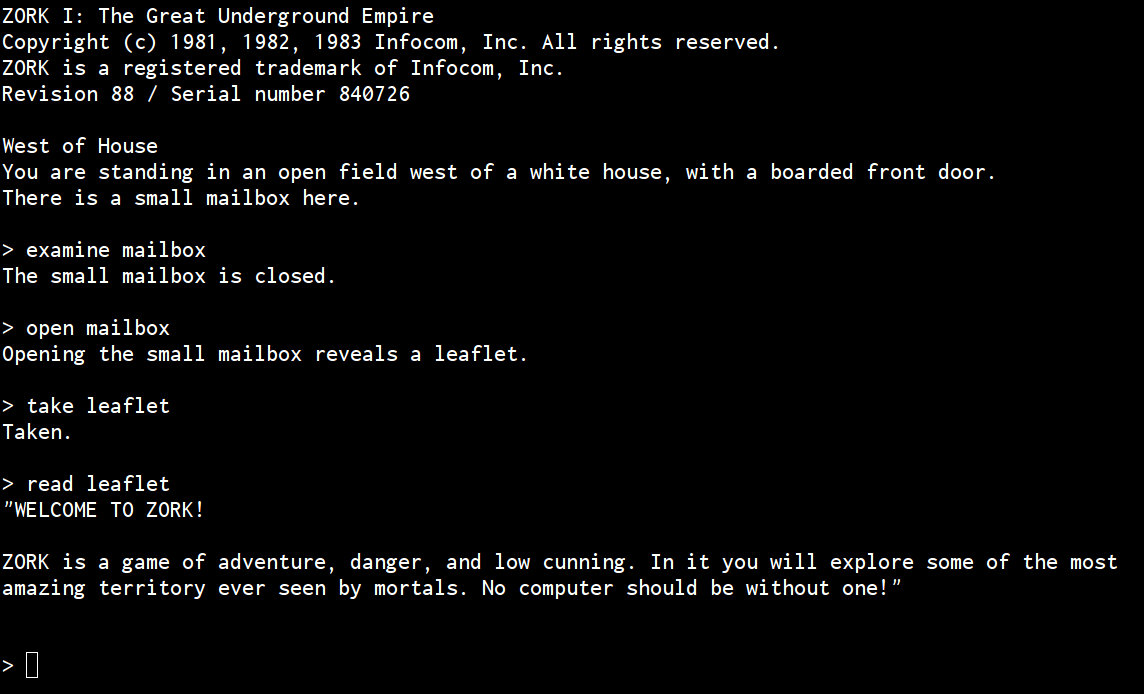
\includegraphics[width=\textwidth]{zork1.png}
    \centering
    \caption{The beginning of a ZORK I session.}
    \label{fig:zork}
\end{figure}

Goal of this thesis is to design, implement, apply and evaluate a framework that allows the creation of tutorials with this teaching approach. In reference to the term \emph{in a nutshell}, which means “to the point” or “short and sweet”, and because the tutorials' user interface resembles a system shell, this framework was called the \emph{Nut Shell}.

\section{Prior work}

\todo{Write.}
%In the technical community, there have been several approaches to create interactive tutorials for command line interfaces.
%
%\emph{Try Ruby} was an interactive online tutorial that would provide an introduction to the Ruby scripting language in the browser. An anonymous programmer called \emph{\_why} first published it at the end of 2005\cite{why05}, to the author's knowledge, this was the first attempt at creating interactive command line tutorials. \_why took the site offline in early 2009, but some members of the Ruby community continued to develop it.
%
%An American company called \emph{Codecademy}\footnote{\url{http://www.codecademy.com/dashboard}} currently deploys several interactive tutorials, which focus on teaching programming in Ruby, Python, JavaScript and PHP. The tutorials consist of multiple exercises, in each of which the users get a piece of unfinished code as well as an exercise and then are supposed to fix or finish the code so that it satisfies some conditions.
%
%\emph{Code School}\footnote{\url{https://www.codeschool.com}} follows a more interactive approach: They offer courses about Ruby, JavaScript, HTML/CSS, R and Git, where the user can enter lines and gets feedback whether that was the solution for the current task.
%
%While these implementations of interactive tutorials pose drastic improvements over classical, static tutorials, they still have several problems:
%
%The presented tutorials are linear: Each task has to be solved to get to the next one.
%
%Furthermore, they do not offer that level of persistence that normal interaction with the command line would: As every entered line is run seperately, the system has no internal state.
%
%While they emulate some editing capabilities regarding command-line editing, to use comfort functions like accessing the command history or using tab-completion is impossible.
%
%The Nut Shell will address all of these shortcomings.

\section{Overview and Organization}

%To allow fast creation of tutorials, we designed a domain specific language tailored to the needs of the tutorial's author.

%The main research question of this thesis is whether this approach is in some way "better" than text tutorials.

The structure of this thesis follows a bottom-up fashion:

\Cref{sec:preliminaries} introduces and defines some of the framework's central topics and terms: \emph{Command line interfaces}, \emph{Terminals}, and related technologies.

\Cref{sec:cli} describes the abstraction layer that communicates with the command line process at the core of each Nut Shell tutorial. It explains and demonstrates techniques for adapting to many different command line interfaces and names the requirements the CLIs need to fulfill.

\Cref{sec:lang} specifies details of the domain specific language \emph{nutsh}, which builds upon the command line abstraction layer to allow simple, fast creation of new Nut Shell tutorials. It describes its syntax and semantics and explains how the language can be interpreted and tested.

\Cref{sec:evaluation} describes application and evaluation of the Nut Shell in an eight-day study with about 120 participants, that compared the new teaching approach with tutorials based on static text, and tried to find out whether the former offers any benefits.

\Cref{sec:implementation} provides an overview of the Nut Shell's implementation and describes usage and installation.

\Cref{sec:nutshexample} on \cpageref{sec:nutshexample} shows an example session of a \emph{bash} tutorial created with the \emph{Nuth Shell}, followed by its source code. To get an impression of the interaction style, it might be beneficial to look at this example before continuing to read.

\section{Notation}
\label{sec:ebnf}

In this thesis, grammars are specified using EBNF as defined in \cite{wirth77}. As a convention, capitalized names represent nonterminal symbols, while lowercase names represent terminal symbols. Tokens are enclosed double quotes or back quotes.

\todo{Short recap of EBNF?}

Grammars are displayed in the following style:

\begin{ebnf}
Grammar     = { Production } .
Production  = production_name "=" [ Expression ] "." .
Expression  = Alternative { "|" Alternative } .
Alternative = Term { Term } .
Term        = production_name | token | Group | Option | Repetition .
Group       = "(" Expression ")" .
Option      = "[" Expression "]" .
Repetition  = "{" Expression "}" .
\end{ebnf}

\chapter{Preliminaries}
\label{sec:preliminaries}

\section{Command line interfaces}
\label{sec:cli}

A \emph{command line interface} (\textsc{CLI}) allows a user to communicate with a computer program by entering lines of text, the \emph{command lines}. This thesis focuses on purely character-based command line interfaces that have no graphical capabilities.

Commonly, interaction with a \textsc{CLI} consists of three phases:

\begin{enumerate}
    \item The program writes a \emph{prompt}, a special character sequence that signals that the program now expects a command.
    \item The user composes a command line. Often, the CLI offers several editing capabilities that make this process more comfortable, like a command history or completion of nonambigious words when pressing \keys{Tab}. To tell the program to execute the command, the user sends a \emph{line feed} character by pressing the \keys{Return} key.
    \item The program executes the command and displays a response. Sometimes, the execution is \emph{interactive} and requires further input. After the command has finished, the first phase starts again.
\end{enumerate}

In this thesis, the examples will use IRB, the \emph{Interactive Ruby Shell}. Ruby is an object-oriented scripting language and, at the basic level, can be used to evaluate arithmetic expressions. \Cref{fig:irb} shows a few iterations of the three phases mentioned above. The characters \texttt{>\->} constitute the prompt, the following characters (set in a bold typeface) are commands the user typed, and the subsequent lines are the program's output.

\begin{figure}[tb]
    \begin{lstlisting}[escapechar=@,frame=shadowbox]
>> @\textbf{2**16}@
=> 65536
>> @\textbf{Math.sqrt(2)}@
=> 1.4142135623730951
>> @\textbf{6*7 == 42}@
=> true
    \end{lstlisting}
    \centering
    \caption{An example IRB session.}
    \label{fig:irb}
\end{figure}

\label{sec:cliexamples}

Another very common command line program is \emph{Bash}, the default system shell on Linux and Mac OS X. \todo{Describe}

\section{Terminal}

In the past, a \emph{computer terminal} was a device for communication with mainframe computers. They read text from the user via a keyboard and displayed the computer's output, first on paper, later on a screen.

Here, when we use the term \emph{terminal}, we mean a modern \emph{terminal emulator}, a program that resembles a computer terminal within an otherwise graphical environment. Inside these terminal emulators, command line programs can be used.

Terminals communicate through sequential streams of characters: They receive characters from the user's keyboard, which they send to the program running inside, and they receive characters back from the program to be displayed on the screen.

\subsection{Escape sequences}

\todo{Explain what escape sequences are, where they come from and list those important for this thesis.}

%A classical computer terminal was the \textsc{VT100}, introduced 1978 by \textsc{Digital Equipment Corporation}. Nowadays, modern terminal emulators mimic its behaviour. The device had a mechanism for doing graphical output: When given special character sequences to display, the terminal performed actions like moving the cursor, deleting characters on the screen or turning graphical modes (underlining, different colors) on and off. Because these sequences “escape” their normal path of being displayed, they are called \emph{escape sequences}. The sequences indeed start with an \emph{escape} character. The \textsc{VT100} supported the escape sequences now defined in ANSI X3.64 (ref), also called the \emph{ANSI escape sequences}.

%\Cref{sec:esc} lists the common escape sequences used today.

\subsection{Readline}

To make text input more comfortable, many CLIs offer a wide range of editing capabilities. They support key combinations for deleting characters, words or whole lines, and often maintain a history of entered commands, so that the user can reuse them later if necessary.

To avoid having to implement these functions themselves, many command line programs use a library called \emph{Readline} \cite{readline}. This library has some default keybindings, which originate from the Emacs text editor. Even if a program does not use Readline directly, many of its bindings have become a de-facto standard for command line editing and thus can be expected to work in a command line environment. \todo{Table of common bindings.}

\chapter{The Command Line Tokenizer}
\label{sec:cliparser}

This chapter describes the construction of the framework's lowest-level component, the \emph{command line tokenizer}, which wraps around the command line process that is to be taught. It watches and modifies its input and output to seperate the different parts of the command line interaction. This creates a layer of abstraction that enables the framework to treat all supported CLIs identically.

In this thesis, the targeted command line process is treated as a black box having input and output streams of Unicode characters. To enable the Nut Shell to check conditions on the user's interaction, it needs to parse the output accordingly.

The interesting parts in this context are the following three, which correspond to the phases described in \cref{sec:cli}:

\begin{enumerate}
    \item Which prompt is displayed to the user?
    \item Which command does he enter?
    \item What is the output of this command?
\end{enumerate}

The main idea here is to use two special \emph{markers}, unique character sequences that do not appear in normal command line interaction, to annotate the output of the process. A suitable choice for those markers are Unicode characters from the \emph{Private Use Area} \cite[p. 558]{unicode6.2}. The different components then can then be recognized by the command line tokenizer. Once the framework is able to understand the program's output, it is able to do two important things:

First, it can check conditions on the different parts. This is necessary to react to the user's commands or to the output.

Second, it can run commands itself in the background, while having access to the same state of the command line system as the user.

\section{Targets}
\label{sec:targets}

The Nut Shell is designed to support many different command line interfaces. Examples of command line programs can be found in \cref{sec:cliexamples}. When we talk about one of these programs, we call it the Nut Shell's current \emph{target}.

For the following mechanisms to work, a command line program needs to have these features:

\begin{itemize}
    \item Freely customizable prompts.
    \item Readline-like keybindings. Mandatory are the following three key combinations:
        \begin{itemize}
            \item \keys{\ctrl+E} has to jump to the end of the line

            \item \keys{\ctrl+U} has to delete the momentarily entered line and puts it in an internal buffer
            
            \item \keys{\ctrl+Y} has to re-insert the content of this buffer
        \end{itemize}
\end{itemize}

All command line programs mentioned in \cref{sec:cliexamples} have those features and thus can be used as \emph{targets}.

\section{High-level architecture}

\todo{Diagram and description of the architecture}

The EBNF grammar shown in this chapter describes how the tokenizer watching the output of the command line process works.

As markers, the Nut Shell simply

The output of a process as it is used in the framework consists of three segments: The prompt (with markers, see next section), the composing of the command (which can include escape sequences for editing, or can consist of several lines), and the command's output. These segments can be repeated. The command output simply consists of non marker characters:

\begin{ebnf}
Output = { PromptWithMarkers CommandComposing CommandOutput } .
CommandOutput = { NonMarker } .
NonMarker = /* every character except marker and marker2 */ .
\end{ebnf}

\section{Recognizing the prompt}

The prompt is the easiest component to recognize. As the prompt of the target process can be changed (by definition, see \cref{sec:targets}), the Nut Shell configures the prompt to start and end with a marker. While parsing, the prompt can now be identified nonambigiously. The markers simply are skipped and are not displayed to the user.

In this part of the grammar, the token we are really interested in is \texttt{Prompt}:

\begin{ebnf}
PromptWithMarkers = marker Prompt marker .
Prompt = { NonMarker } .
\end{ebnf}
%
This approach has a downside: In some command line programs it is possible to change the prompt from within the program. If the user tries to change the prompt himself, this method will no longer work.

To add support for a new command line program to the Nut Shell, one has to create a profile that specifies which options and commands are necessary to configure the prompt so it begins and ends with markers.

\todo{Example configurations for IRB and bash.}

\section{Recognizing the command}

When the user enters characters with his keyboard, normally, these characters are immediately displayed on the screen. This means that in the phase of entering a command, the input of the underlying process equals its output.

Unfortunately, this is only true for visible characters. While editing the command line, a user may use Readline's key bindings or other shell builtin key combinations that modify the currently entered command in unusual ways. These make it hard for the framework to recognize which command he entered, as parts of the entered characters could have been deleted or otherwise have been changed. To solve this, the Nut Shell uses the following mechanism to repeat the entered line between two markers before it is sent:

When the user is done editing the command, wants to run it and produces a \emph{line feed} character by pressing \keys{Return}, the Nut Shell does not send this character to the process. Instead, using the Readline key bindings, it proceeds in the following way:

\begin{enumerate}
    \item The cursor is positioned at the end of the line using \keys{\ctrl+E}. This is necessary as the user could have positioned the cursor somewhere inside the command as well.
    \item A \emph{space} character is inserted. This prevents problems when the command was completely empty before, as the following step wouln't do anything in this case:
    \item The whole line is deleted and put into an internal buffer using \mbox{\keys{\ctrl+U}}.
    \item A marker is inserted and immediately deleted afterwards, so it does not end up in the command later.
    \item The deleted command is re-inserted using \keys{\ctrl+Y}.
    \item Another marker is inserted and deleted.
    \item The \emph{space} character that was inserted in step 2 is deleted.
    \item Finally, a \emph{line feed} character is written to the process to start exection of the command.
\end{enumerate}

This is the whole sequence as it is sent to the process:

\begin{quote}
    \keys{\ctrl+E} \keys{space} \keys{\ctrl+U} marker \keys{backspace} \keys{\ctrl+Y} marker \keys{backspace} \keys{backspace} \keys{\return}
\end{quote}

Because \keys{\ctrl+Y} repeats the whole command as the user intended to run it, it now appears in the output cleanly framed by the two markers. The screen's content, however, looks the same to the user.

\begin{table}[tb]
    \centering
    \caption{Example of the command marker technique.}
    \label{tab:cmdmarking}
    \begin{tabular}{l|l|l|l}
        Keystrokes & Input & Output & Screen content \\
        \hline
        & & \texttt{>>␣} & \texttt{>>␣\cursor} \\
        \keys{1} \keys{-} \keys{1} & \texttt{1-1} & \texttt{1-1} & \texttt{>>␣1-1\cursor} \\
        \keys{\arrowkeyleft} & \texttt{\escape{[}[D} & \texttt{\escape{H}} & \texttt{>>␣1-\invert{1}} \\
        \keys{backspace} & \texttt{\escape{H}} & \texttt{\escape{H}} & \texttt{>>␣1\invert{-}1} \\
        & & \texttt{\escape{[}[1P} & \texttt{>>␣1\invert{1}} \\
        \keys{{+}} & \texttt{+} & \texttt{+} & \texttt{>>␣1+\cursor} \\
        & & \texttt{1} & \texttt{>>␣1+1\cursor} \\
        & & \texttt{\escape{H}} & \texttt{>>␣1+\invert{1}} \\
        \keys{\return} & \texttt{\escape{E}} & \texttt{\escape{[}[C} & \texttt{>>␣1+1\invert{ }} \\
        & \texttt{␣} & \texttt{␣} & \texttt{>>␣1+1␣\invert{ }} \\
        & \texttt{\escape{U}} & \texttt{\escape{H}\escape{H}\escape{H}\escape{H}} & \texttt{>>␣\invert{1}+1␣} \\
        & & \texttt{\escape{[}[K} & \texttt{>>␣\invert{ }} \\
        & \texttt{\{marker\}} & \texttt{\{marker\}} & \texttt{>>␣\{marker\}\invert{ }} \\
        & \texttt{\escape{H}} & \texttt{\escape{H}\escape{[}[K} & \texttt{>>␣\invert{ }} \\
        & \texttt{\escape{Y}} & \texttt{1+1␣} & \texttt{>>␣1+1␣\invert{ }} \\
        & \texttt{\{marker\}\escape{H}} & \texttt{\{marker\}\escape{H}\escape{[}[K} & \texttt{>>␣1+1␣\invert{ }} \\
        & \texttt{\escape{H}} & \texttt{\escape{H}\escape{[}[K} & \texttt{>>␣1+1\invert{ }} \\
    \end{tabular}
\end{table}

\Cref{tab:cmdmarking} demonstrates the technique. The first column lists the user's keystrokes, the second one contains the characters sent to the process, the third one contains the output of the process, and the final one shows the current content of the screen. The gray rectangle indicates the cursor position. In the example, the user enters \texttt{1-1}, and then replaces the \texttt{-} character with a \texttt{+} using arrow keys and \emph{backspace}. From the output so far, it is hard to recognize the actual command (which is displayed on the screen).

\todo{Add line numbers to the table, explain the escape codes.}

When the user presses \emph{return}, the described sequence is sent to the process, and when reading the “Output” column, the correct command \texttt{1+1} appears cleanly between the two markers. Ater the first marker, there are some deletion characters in the output (they depend on the concrete command line program, but come from a fixed character set), and before the second marker there's always a space character. By removing these, the exact command the user wanted to enter is left.

In general, for the tokenizer, the composing sequence has two phases: In the first one, the actual command line composing takes place. In the second one, the current line is deleted and reprinted as described above. The interesting part here is \texttt{Command}:

\begin{ebnf}
ComposeAndRepeat = LineComposing LineRepetition .
LineComposing = { NonMarker } .
LineRepetition = Deletition Marker Deletion Command
    space Marker Deletion "\r" .
Deletition = { DeletitionCharacter } .
DeletitionCharacter = ^H | ^[[K | ^[[1P | ... .
Command = { NonMarker } .
\end{ebnf}

\subsection*{Multi-line commands}

When the user wants to executes a command, some \textsc{CLI}s check whether this command is complete. When it is not, they do not execute the command, but give him the possibility to complete it instead. In this case, the CLI usually displays a secondary prompt.

\todo{Example of such an incomplete command, with a missing closing bracket.}

The framework inserts a second kind of marker in the secondary prompt, too, so that it can be recognized and differentiated from a normal prompt.

After the previously described line repetition, the tokenizer looks at the next character---if it is a secondary-prompt-marker, it knows another composing-and-repeating step will follow, as the user will now type a second line:

\begin{ebnf}
SecondaryPromptWithMarkers = marker2 Prompt marker2 .
CommandComposing = ComposingAndEcho
    [ { SecondaryPromptWithMarkers ComposingAndEcho } ] .
\end{ebnf}
%
When no secondary prompt follows, all occurrences of the \texttt{Command} token are appended to get the full command.

\chapter{The \emph{nutsh} Language}
\label{sec:lang}

To enable authors to write tutorials for the Nut Shell quickly, the framework supports a new \emph{domain-specific programming language} (\textsc{DSL}). This language is called \emph{nutsh}, a contraction of “Nut Shell”, which also serves as the filename extension. Files written in the \emph{nutsh} language represent “lessons”, self-contained teaching units.

%The language contains syntactic structures that support often-used semantical statements. It provides mechanisms to reuse code snippets to minimize redundance.

%The language is string-based, the only data type is a string of Unicode characters, this keeps the language minimal. \emph{nutsh} does not have variables, which makes the language functional.

The following sections specify the language's lexical and syntactical elements in \textsc{EBNF} as defined in \cref{sec:ebnf} and describe their semantics.

Lesson files should be as easy to read and to write as possible. Because of this, \emph{nutsh} uses a syntax that is close to other languages potential users will already know. In this case, it resembles the syntax of C, with some influences of Google Go \cite{google13}, for example the definition of string literals and the syntax of \texttt{if} clauses.

Another design goal was to keep the language as small as possible, while making it powerful enough for the intended purpose. For this reason, the only data type is a string of Unicode characters, and it has no variables.

\section{Lexical elements}

\minisec{Comments}

\emph{nutsh} has two types of comments, as they exist in C-like languages: \emph{Line comments} start with \texttt{//} and stop at the end of the line, \emph{block comments} start with \texttt{/*} and end with \texttt{*/}. Comments act as white space and are ignored otherwise.

\minisec{White space}

Whites space (newlines, carriage returns, tab and space characters) seperates tokens but has no further meaning.

\minisec{Identifiers}

Identifiers serve as names that can be used for functions. An identifier is a nonempty sequence of alphanumeric characters.

\begin{ebnf}
Identifier = alnum_char { alnum_char } .
\end{ebnf}

\minisec{Keywords}

\emph{nutsh} uses the following keywords, which may not be used as identifiers:

\begin{quote}
    \texttt{break}\hspace{0.5em}
    \texttt{def}\hspace{0.5em}
    \texttt{else}\hspace{0.5em}
    \texttt{if}\hspace{0.5em}
    \texttt{prompt}\hspace{0.5em}
    \texttt{return}
\end{quote}

\minisec{Operators and delimiters}

The following character sequences have special meanings in \emph{nutsh}:

\begin{quote}
    \texttt{=\~}\hspace{1em}
    \texttt{==}\hspace{1em}
    \texttt{||}\hspace{1em}
    \texttt{,}\hspace{1em}
    \texttt{!}\hspace{1em}
    \texttt{(}\hspace{1em}
    \texttt{)}\hspace{1em}
    \texttt{\{}\hspace{1em}
    \texttt{+}\hspace{1em}
    \texttt{\}}\hspace{1em}
    \texttt{\&\&}
\end{quote}

\minisec{String Literals}

There are two types of string literals, which have the same syntax as in Go: \emph{raw string literals} and \emph{interpreted string literals}. Raw string literals are enclosed with back quotes (\texttt{\`}). They may contain any character except the back quote; the characters are interpreted literally. Interpreted string literals are enclosed with double quotes (\texttt{"}) and may contain backslash escapes; Their exact definition can be found in the Go specification \cite{google13}. \todo{Examples of interpreted strings?}

\begin{ebnf}
string = raw_string | interpreted_string .
raw_string = "`" { unicode_char } "`" .
interpreted_string = `"` { unicode_char | escaped_char |
    byte_value } `"` .
\end{ebnf}

\section{Expressions}

\minisec{String Expressions}

The \emph{nutsh} language makes strong use of strings (\texttt{"foo"}). String expressions can be concatenated (\texttt{"foo"+"foo"} has the same value as \texttt{"foofoo"}) and be checked for equality (\texttt{"foo" == "foo"}). Additionally, one can check whether a string matches a regular expression (\texttt{"foo" =~ "f.."}).\footnote{Using the syntax of the regular expression parsing library \emph{RE2} as described here: \url{https://code.google.com/p/re2/wiki/Syntax}} Every string can be interpreted as a truth value, which is \emph{false} for an empty string and \emph{true} otherwise. The common logic operators (\texttt{!} for \emph{not}, \texttt{\&\&} for \emph{and}, and \texttt{||} for \emph{or} are defined accordingly. They return the (arbitrary) nonempty string \texttt{"true"} as a truth value.

\begin{ebnf}
StringExpression =
    string | Call | StringExpression Operator StringExpression |
    "!" StringExpression | "(" StringExpression ")" .

Operator = "+" | "==" | "=~" | "&&" | "||" .
\end{ebnf}

\minisec{Operator precedence}

String concatenation binds strongest, followed by the two comparison operators, logical \emph{and}, and finally logical \emph{or}. Operators bind from left to right: \texttt{a OP b OP c} has the same meaning as \texttt{(a OP b) OP c}.

\minisec{Calls}

\emph{nutsh} knows \emph{functions}, which can be called by specifying the correct number of arguments. If a function takes no arguments, the brackets can be omitted. As a special case, a string on its own also acts as a function call, see the following section.

\begin{ebnf}
Call = identifier [ "(" [ StringExpressions ] ")" ] | string .
StringExpressions = StringExpression { "," StringExpression } .
\end{ebnf}

\section{Built-in functions}

A central command is the output of explanation text. This text will be displayed indented and highlighted in a different color.

\begin{nutsh}
say("This is explaining text.")
\end{nutsh}
%
Because this command is used so often, it can be abbreviated to:

\begin{nutsh}
"This is the short form."
\end{nutsh}
%
The \texttt{say} function supports two ways of highlighting parts of the text: Text enclosed in back quotes will be displayed in a second color, text enclosed in asterisks in a third. As a convention, back quotes are used to mark parts of commands or file names, and asterisks are used to emphazise parts of a sentence. These conventions have been adopted from John Gruber's Markdown.\footnote{\url{http://daringfireball.net/projects/markdown/syntax}}

The \texttt{run} function executes a command in the target process, it takes a command line to be executed as an argument. The value of this statement is the command's output.

\begin{nutsh}
run("1+1")
\end{nutsh}

\section{Statements}
\label{sec:statements}

\minisec{Blocks}

A \emph{block} is a sequence of lines:

\begin{ebnf}
Block = "{" { Line } "}" .
Line = IfStatement | PromptStatement | NestingStatement | Call .
\end{ebnf}

\minisec{If statements}

If the conditional expression of an \texttt{if} statement evaluates to \emph{true}, the first block is evaluated, otherwise the (optional) second block. There are no brackets around the condition.

\begin{ebnf}
IfStatement = "if" StringExpression Block ( "else" Block ) .
\end{ebnf}
%
This example checks a string for equality with itself and prints an according message:

\begin{nutsh}
if "test" == "test" {
    "Everything is OK."
} else {
    "Wait, what?"
}
\end{nutsh}

\minisec{Prompt statements}

The prompt statement is a central element of \emph{nutsh}'s syntax. It has the semantic of an endless loop, in which a command is read from the user at the beginning of each pass. It can be left with a \texttt{break} statement.

\begin{ebnf}
PromptStatement = "prompt" Block .
\end{ebnf}
%
There are two builtin functions called \texttt{command} and \texttt{output}, that correspond to the user's latest command and its output. When no prompt has occurred yet, they return empty strings.

In this example, the user is asked to enter a command that has the output “42”. When he obeys, the prompt loop is left with a \texttt{break} statement, otherwise he has to try again:

\begin{nutsh}
"Please calculate the product of 6 and 7."

prompt {
    if output == "42" {
        break
    } else {
        "Please try again."
    }
}

"Well done!"
\end{nutsh}

\minisec{Function definition}

To define a new function, the \texttt{def} keyword is used, followed by the name of the function, optional arguments and a block. The brackets around the arguments can be omitted if a function has no arguments:

\begin{ebnf}
Definition = "def" identifier [ Arguments ] Block .
Arguments = "(" [ identifier { "," identifier } ] ")" .
\end{ebnf}
%
As an example, we define a function that prints its argument twice:

\begin{nutsh}
def say_twice(text) {
    say(text)
    say(text)
}

say_twice("Hey!")
\end{nutsh}

\minisec{Nesting statements}

Sometimes, the same set of conditions needs to be checked for a group of prompt statements. In this case, nesting statements can be used. They consist of one or more function calls, followed by a block.

\begin{ebnf}
NestingStatement = Calls Block .
Calls = Call { "," Call } .
\end{ebnf}
%
At each pass of a prompt loop, after the command has been read from the user, the specified parent functions are called. There can be more than one level of nesting -- the outmost parent functions are called first.

In this example, a function is defined that prints a message when the user enters a command that contains “help”. For two \texttt{prompt} statements, a nesting statement is defined to call this function. Now every time the user enters a command in these two prompt loops, the function is called.

\begin{nutsh}
def respond_to_help {
    if command =~ "help" {
        "Sorry, you're on your own."
    }
}

respond_to_help {
    prompt {
        // break condition ...
    }
    prompt {
        // break condition ...
    }
}
\end{nutsh}
%
For another example of this syntax, refer to the implementation of the example lesson in \cref{sec:nutshexample}, starting on \cpageref{lst:compress}.

\section{Top level structure}

A \emph{nutsh} file consists of several function definitions and other \texttt{Line} instances (\texttt{if}-, \texttt{prompt}- and nesting statements in addition to calls, see \cref{sec:statements}). Thus, function definitions can only appear at the top level to avoid redefinitions in different scopes, which would lead to name masking problems and a much higher complexity.

\begin{ebnf}
Lesson = { Definition | Line } .
\end{ebnf}

\section{Parsing}

\emph{nutsh} uses a standard YACC parser, which is described in more detail in \cref{sec:implementation}. The parser creates a \emph{syntax tree} whose nodes have a string value and zero or more child nodes. For leaf nodes, the string value represents the lexical value, for inner nodes, it represents the node's type.

\todo{Examples of parsed code snippets?}

\section{Interpretation}

\todo{To write.}

%A node's values can always be calculated from its children's values. We call this a \emph{synthesized attribute}. As all attributes can be synthesized, \emph{nutsh}'s gramar is said to be \emph{S-attributed}. This makes an evaluation of the syntax tree especially easy, as the interpreter can now travel through the tree in a bottom-up manner.
%
%While traversing through the syntax tree, the interpreter keeps track of the encountered nesting statements.
%
%When a function definition is encountered, the definition node along with its children is added to the symbol table.
%
%When a \texttt{prompt} node is encountered, the \emph{command line parser} is used to prompt the user for a command. The command and it's output are saved so they can be accessed when the \texttt{input} and \texttt{output} functions are called.
%
%(ref: dragon)
%
%(State)

\section{Automated testing}


As the author of a tutorial, one wants to verify that all the lessons work correctly. The framework provides a function for automated testing of correctness, so one does not have to enter all the required commands by hand.

To help with this, the framework provides the builtin function \texttt{expect}, which expresses the assumption of the author that if a user were to enter the supplied argument as a command in the innermost surrounding \texttt{prompt} statement, the \texttt{expect} statement would be reached.

In this example, the user is asked to reverse a given string. The \texttt{expect} lines give two different ways to achieve it---both should work. There's also an \texttt{expect} command that should \emph{not} lead to an evaluation of the first block:

\begin{nutsh}
run("text = 'stressed'")
"Reverse the content of `text` and save it in `text2`!"
prompt {
    if test("text2 == 'desserts'") {
        "You did it!"
        expect("text2 = text.reverse")
        expect("text.reverse!; text2 = text")
        break
    } else {
        expect("text2 = 'somethingdifferent'")
    }
}
\end{nutsh}

The testing algorithm first collects all \texttt{expect} statements and creates a reference for each of them in the nearest \texttt{prompt} statement around the statement.

It then starts interpreting the file like normally, but when a \texttt{prompt} statement is encountered, instead of querying the user for a command, one of the unreached associated \texttt{expect} commands is used. When the respective \texttt{expect} statement is reached, the statement is marked as \emph{reached}. When the end of the prompt loop is reached, and the \texttt{expect} has not been reached, an error is printed and the test is aborted. At the end of the file, if there are any unreached \texttt{expect}s left, the lesson is restarted.

By convention, when a prompt is encountered whose expects are all reached, the first one is used. Thus, the first expect in each prompt should be one that leads to a \texttt{break} statement to ensure the testing algorithm terminates.

\chapter{Application and Evaluation}
\label{sec:evaluation}

To find out whether the teaching method provided by the Nut Shell has any advantages compared to traditional teaching methods, we created an example tutorial and conducted a two-week course with a subsequent survey.

\section{Setting}

The \textit{Braunschweig University of Technology} has been organizing preparatory computer science courses for freshman students since 2003. This course teaches how to use UNIX-like operating systems and accompaning tools for program creation.

Until now, these topics were tought by handing out exercises on paper, which the students could work on in computer pools. For support, student assistants were provided, with about one assistant per 25 students.

In the fall semester 2013--2014, 150 students enrolled in the course. For this study, the students were split into two groups: Two thirds of the students were randomly selected to use the Nut Shell, the remaining one third worked with the previously used exercises on paper. The groups worked in two separate rooms. Each day, there were three time slots of 75 minutes each, to which the students were assigned in equal parts. The course spanned over eight days, not including a weekend and a day off.

The course roughly covered the these topics: The \textsc{UNIX} file system and how to manipulate it; various text editors like Vim, Emacs, and Gedit; process management; command line tools for text manupulation like \texttt{grep}, \texttt{sort}, or \texttt{patch}; various shell mechanism like output redirection and the command history; shell scripts; automatition with Makefiles; accessing remote servers with \textsc{SSH}; typesetting documents with \LaTeX; understanding and repairing programs written in \textit{Java}; and version control with \textit{Git}.

The newly created \textit{Nut Shell} tutorial kept these topics and their order. The material was divided into 30 invidiual lessons, each of which covered one specific topic. Each day, new lessons were made available. In total, the tutorial contained 2875 lines of \textit{nutsh} code. It took about 30 hours to write and test the lessons. For an example lesson, refer to \cref{sec:nutshexample}.

\section{Style}

The basic structure in the Nut Shell tutorial when introducing new concepts is the following: First, a general problem is stated. The method or tool for solving these class of problems is presented using a simple example, in which the user is guided exactly what to do. After that follow several problems of increasing difficulty which the user has to solve on his own. Finally, some advanced concepts and ideas are mentioned, and the user is given some free room to experiment with those. A clear signal is communicated that the user can use to continue.

Often, goals are stated but how to achieve it is up to the user. This has to be realized by testing against \texttt{output()} and \texttt{run()} statements. At several occasions, the user can choose among several paths to continue or can determine in which order to learn about several topics. These structures are supposed to give the user a feeling of autonomy and control.

For better illustration and for a more entertaining experience, the lessons introduce several real-world metaphors for abstract concepts. For example, in a lesson about the compression of files, the user is confronted with a directory named \textit{fridge} and a large file named \textit{elephant} and is asked to put the elephant in the fridge.\footnote{This is a reference to the old joke “How do you put an elephant into a fridge? -- Open the fridge, put in the elephant, and close the door.”} To complete this task, the file has to be compressed.

\section{Survey}

After the sixth day, an online survey was conducted whithin both groups. In the first part, the following general questions were asked (in German):

\begin{itemize}
    \item What is your course of studies?
    \item Did you use the Nut Shell or the paper exercises?
    \item On a range from 1 (not at all) to 10 (entirely), how much do you agree to the following statements?
        \begin{enumerate}
            \item I had previous knowledge about the command line.
            \item The tutorial was fun.
            \item I learned a lot in the tutorial.
            \item The exercises were too hard.
            \item I had enough time to complete the exercises.
            \item I think the material is relevant for my further education.
            \item I would recommend the tutorial to others.
        \end{enumerate}
    \item How many times did you have to ask for help per day?
\end{itemize}

The second part of the survey was a test with 11 questions about different topics of the tutorial, in an attempt to quantify how much the participants learned. The following questions were provided by a person who was uninvolved with and unaware of the content of the Nut Shell lessons to avoid a bias which could have led to asking questions we knew the Nut Shell explained well. For evaluation, each answer was marked with either 0 points (no or wrong answer), 0.5 points (correct parts), or 1 points (complete and correct answer).

\begin{enumerate}
    \item How do you create the directory \texttt{abc.txt}?
    \item How do you copy the file \texttt{abc.txt} to the directory \texttt{xyz}?
    \item How can you obtain more information about the command \texttt{mv}?
    \item Name at least two ways to look at the content of the file \texttt{abc.txt}.
    \item What do you use the command \texttt{ln} for?
    \item Output all lines of the file \texttt{abc.txt} that contain the Text "Hallo".
    \item What is the variable \texttt{PS1} used for?
    \item What do you use \texttt{>} and \texttt{>>} for and how do they differ?
    \item How dou you archive and compress all files with the ending "123" in the current directory?
    \item What is the file \texttt{~/.bashrc} used for?
    \item You don't want to type \texttt{ls -alR} all the time, but create a short hand form. Which possibilities do you have and what is the corresponding command?
    \item What are pipes used for and how do you use them? Write an example command.
\end{enumerate}

The third batch of the questions was only given to the students who had used the Nut Shell. It is intended to assess strenghts and weaknesses of the created tutorial:

\begin{enumerate}
    \item The Nut Shell did a good job explaining new material.
    \item When I encountered problems, the Nut Shell gave helpful hints.
    \item The exercises were helpful to understand the topics on hand.
    \item When attending another course, I would like to use the Nut Shell again.
\end{enumerate}

\section{Results}

For the Survey's first part, there were 64 answers in total. 52 of the participants specified they had used the Nut Shell, 11 of them had used the exercise sheets. \Cref{fig:general} juxtaposes the answers to the general questions of both groups in the form of a box plot: The circle marks the median of the answers to each question, the box contains 50\% of the answers, the whiskers reach from the minimum to the maximum answer. According to the participants, the Nut Shell users had significantly more fun and had the impression of having learned more than the paper exersice users. While there is a slight evidence that the Nut Shell users found the course easier, had less time, and thought of the topics to be more relevant, these differences are not statistically meaningful.

\begin{figure}[p]
    \begin{tikzpicture}[trim axis left, trim axis right]
        \begin{axis}[
                boxplotcompare style,
                ytick={1,2,3,4,5,6,7},
                yticklabels={Prior knowl., Fun, Learned a lot, Too hard, Enough time, Relevant, Recommend},
                boxplot,
                y dir=reverse,
                height=\textheight,
                width=\textwidth,
                xmin=0.5,
                xmax=10.5,
                xmajorgrids,
                ymin=0,
                ymax=8,
            ]

            \addlegendimage{area legend, fill=white, draw=black}
            \addlegendentry{Exercise Sheets};
            \addlegendimage{area legend, fill=gray, draw=black}
            \addlegendentry{Nut Shell};

            \addplot[
                forget plot,
                rshift,
                boxplot prepared={
                    lower whisker =1,
                    lower quartile=1,
                    median        =2,
                    upper quartile=4.25,
                    upper whisker =10,
                },
            ] coordinates {};
            \addplot[
                lshift,
                boxplot prepared={
                    lower whisker =1,
                    lower quartile=1,
                    median        =1.5,
                    upper quartile=2.25,
                    upper whisker =3,
                },
            ] coordinates {};

            \addplot[% fun
                forget plot,
                rshift,
                boxplot prepared={
                    lower whisker =3,
                    lower quartile=7,
                    median        =9,
                    upper quartile=10,
                    upper whisker =10,
                },
            ] coordinates {};
            \addplot[
                lshift,
                boxplot prepared={
                    lower whisker =6,
                    lower quartile=7,
                    median        =8,
                    upper quartile=8,
                    upper whisker =10,
                },
            ] coordinates {};

            \addplot[% learn
                forget plot,
                rshift,
                boxplot prepared={
                    lower whisker =5,
                    lower quartile=8,
                    median        =9,
                    upper quartile=9.25,
                    upper whisker =10,
                },
            ] coordinates {};
            \addplot[
                lshift,
                boxplot prepared={
                    lower whisker =5,
                    lower quartile=7,
                    median        =7.5,
                    upper quartile=9,
                    upper whisker =10,
                },
            ] coordinates {};

            \addplot[% too hard
                forget plot,
                rshift,
                boxplot prepared={
                    lower whisker =1,
                    lower quartile=3,
                    median        =4,
                    upper quartile=5,
                    upper whisker =9,
                },
            ] coordinates {};
            \addplot[
                lshift,
                boxplot prepared={
                    lower whisker =2,
                    lower quartile=2.75,
                    median        =4.5,
                    upper quartile=5.25,
                    upper whisker =7,
                },
            ] coordinates {};

            \addplot[% enough time
                forget plot,
                rshift,
                boxplot prepared={
                    lower whisker =3,
                    lower quartile=7,
                    median        =9,
                    upper quartile=10,
                    upper whisker =10,
                },
            ] coordinates {};
            \addplot[
                lshift,
                boxplot prepared={
                    lower whisker =3,
                    lower quartile=8.75,
                    median        =10,
                    upper quartile=10,
                    upper whisker =10,
                },
            ] coordinates {};

            \addplot[% relevant
                forget plot,
                rshift,
                boxplot prepared={
                    lower whisker =5,
                    lower quartile=7,
                    median        =8,
                    upper quartile=9,
                    upper whisker =10,
                },
            ] coordinates {};
            \addplot[
                lshift,
                boxplot prepared={
                    lower whisker =5,
                    lower quartile=6.75,
                    median        =7.5,
                    upper quartile=8.25,
                    upper whisker =10,
                },
            ] coordinates {};

            \addplot[% recommend
                forget plot,
                rshift,
                boxplot prepared={
                    lower whisker =4,
                    lower quartile=8,
                    median        =9,
                    upper quartile=10,
                    upper whisker =10,
                },
            ] coordinates {};
            \addplot[
                lshift,
                boxplot prepared={
                    lower whisker =6,
                    lower quartile=7.75,
                    median        =9,
                    upper quartile=10,
                    upper whisker =10,
                },
            ] coordinates {};
        \end{axis}
    \end{tikzpicture}
    \centering
    \caption{Answers to general questions.}
    \label{fig:general}
\end{figure}

\Cref{fig:help} shows the answers to the question regarding how many times per day the participant needed support from a student assistant. Clearly, the Nut Shell users needed less help.

\begin{figure}[tb]
    \begin{tikzpicture}[trim axis left, trim axis right]
        \begin{axis}[
                boxplotcompare style,
                ytick={1},
                yticklabels={help/day},
                boxplot,
                y dir=reverse,
                height=0.32\textwidth,
                width=\textwidth,
                xmin=-0.5,
                xmax=10.5,
                xmajorgrids,
                ymin=0.2,
                ymax=1.5,
            ]

            \addlegendimage{area legend, fill=white, draw=black}
            \addlegendentry{Exercise Sheets};
            \addlegendimage{area legend, fill=gray, draw=black}
            \addlegendentry{Nut Shell};

            \addplot[
                forget plot,
                rshift,
                boxplot prepared={
                    lower whisker =0,
                    lower quartile=1,
                    median        =1.5,
                    upper quartile=3,
                    upper whisker =10,
                },
            ] coordinates {};
            \addplot[
                lshift,
                boxplot prepared={
                    lower whisker =1,
                    lower quartile=2,
                    median        =4,
                    upper quartile=5.5,
                    upper whisker =10,
                },
            ] coordinates {};
        \end{axis}
    \end{tikzpicture}
    \centering
    \caption{Times the participants had to ask for help per day.}
    \label{fig:help}
\end{figure}

\Cref{fig:test} shows the distribution of test scores. The hightest achievable score was $12$. The exercise sheet group achieved a slightly higher score.

\begin{figure}[tb]
    \begin{tikzpicture}[trim axis left, trim axis right]
        \begin{axis}[
                boxplotcompare style,
                ytick={1},
                yticklabels={Score},
                boxplot,
                y dir=reverse,
                height=0.32\textwidth,
                width=\textwidth,
                xmin=-0.5,
                xmax=12.5,
                xmajorgrids,
                ymin=0.2,
                ymax=1.5,
            ]

            \addlegendimage{area legend, fill=white, draw=black}
            \addlegendentry{Exercise Sheets};
            \addlegendimage{area legend, fill=gray, draw=black}
            \addlegendentry{Nut Shell};

            \addplot[
                forget plot,
                rshift,
                boxplot prepared={
                    lower whisker =3,
                    lower quartile=5,
                    median        =6,
                    upper quartile=7.5,
                    upper whisker =12,
                },
            ] coordinates {};
            \addplot[
                lshift,
                boxplot prepared={
                    lower whisker =3,
                    lower quartile=5.75,
                    median        =7,
                    upper quartile=8.375,
                    upper whisker =9,
                },
            ] coordinates {};
        \end{axis}
    \end{tikzpicture}
    \centering
    \caption{Points that the participants got in the test.}
    \label{fig:test}
\end{figure}

\Cref{fig:meta} shows the answers to the Nut Shell related questions. The initial explanations as well as the exercises received high scores, with a median of $9$, the tips for solving the exercises received a median score of $7$. Over half of the participants would like to use the Nut Shell again for a future tutorial.

\begin{figure}[tb]
    \begin{tikzpicture}[trim axis left, trim axis right]
        \begin{axis}[
                boxplotcompare style,
                ytick={1,2,3,4},
                yticklabels={Explanations, Tips, Exercises, Use again},
                boxplot,
                y dir=reverse,
                height=0.3\textheight,
                width=\textwidth,
                xmin=0.5,
                xmax=10.5,
                xmajorgrids,
                ymin=0,
                ymax=5,
            ]

            \addplot[%explanation
                fill=gray,
                boxplot prepared={
                    lower whisker =5,
                    lower quartile=8,
                    median        =9,
                    upper quartile=10,
                    upper whisker =10,
                    box extend=0.6,
                },
            ] coordinates {};
            \addplot[%help
                fill=gray,
                boxplot prepared={
                    lower whisker =2,
                    lower quartile=5,
                    median        =7,
                    upper quartile=8,
                    upper whisker =10,
                    box extend=0.6,
                },
            ] coordinates {};
            \addplot[%exercises
                fill=gray,
                boxplot prepared={
                    lower whisker =4,
                    lower quartile=7,
                    median        =9,
                    upper quartile=10,
                    upper whisker =10,
                    box extend=0.6,
                },
            ] coordinates {};
            \addplot[%again
                fill=gray,
                boxplot prepared={
                    lower whisker =5,
                    lower quartile=8,
                    median        =10,
                    upper quartile=10,
                    upper whisker =10,
                    box extend=0.6,
                },
            ] coordinates {};
        \end{axis}
    \end{tikzpicture}
    \centering
    \caption{Answers to Nut Shell related questions.}
    \label{fig:meta}
\end{figure}

\Cref{fig:participants} shows the number of participants per day in both groups.

\begin{figure}[tb]
    \begin{tikzpicture}[trim axis left, trim axis right]
        \pgfplotstableread{ % Read the data into a table macro
            Label	Slot1	Slot2	Slot3	a	b	c
            1	29	26	25	15	15	15
            2	25	28	24	9	15	5
            3	30	25	16	9	10	15
            4	24	22	16	9	12	5
            5	25	19	11	6	10	1
            6	0	0	0 	0	0	0
            7	0	0	0 	0	0	0
            8	23	28	12	9	11	2
            9	25	23	19	9	6	0
            10	0	0	0 	0	0	0
            11	25	20	6 	10	1	0
        }\datatable

        \begin{axis}[
                width=\textwidth,
                ybar stacked,
                ymin=0,
                xmin=-1,
                xmax=11,
                xtick=data,
                xticklabels from table={\datatable}{Label},
                xlabel=Day,
                ylabel=Participants,
                ymajorgrids,
            ]

            \addlegendimage{area legend, fill=white, draw=black}
            \addlegendentry{Exercise Sheets};
            \addlegendimage{area legend, fill=gray, draw=black}
            \addlegendentry{Nut Shell};

            \addplot [fill=gray, bar shift=-.2cm] table [y=Slot1, x expr=\coordindex] {\datatable};    % Plot the "First" column against the data index
            \addplot [fill=gray, bar shift=-.2cm] table [y=Slot2, x expr=\coordindex] {\datatable};
            \addplot [fill=gray, bar shift=-.2cm] table [y=Slot3, x expr=\coordindex] {\datatable};

            \resetstackedplots

            \addplot [fill=white, bar shift=.2cm] table [y=a, x expr=\coordindex] {\datatable};
            \addplot [fill=white, bar shift=.2cm] table [y=b, x expr=\coordindex] {\datatable};
            \addplot [fill=white, bar shift=.2cm] table [y=c, x expr=\coordindex] {\datatable};
        \end{axis}
    \end{tikzpicture}
    \centering
    \caption{Number of participants per day. Days 6 and 7 were a weekend, there was no course on day 10. From bottom to top, the bar's segments represent first, second and third time slot.}
    \label{fig:participants}
\end{figure}

\section{Discussion}

The small number of participants in the exercise sheet group that were left after day 8 were a problem. The results are likely to be warped, as just those participants who had fun and learned something stayed, which explains why the scores are relatively close to each other.

That is why only the evaluation of the numbers of participants over time is really meaningful. In this case, 63.8\% of the Nut Shell users stayed until the last day. Of the exercise sheet users, only 24.4\% stayed. According to the course's organizers and former assistants, this last number is indeed typical and representative for the course. This could hint that the Nut Shell lesson motivated the students more to attend to the course. For whichever reason this happened: From a lecturer's perspective, this result of keeping the students motivated to attend, is highly gratifying.

Another positive result is the lowered demand for external help the Nut Shell users had. In this case, the Nut Shell users on average asked half the number of questions compared to the exercise sheet group. On the one hand, this is pleasing for the students theirselves, as they can learn more independently---for example, from home, where no external help is available. On the other hand, the number of required student assistants can be lowered, leading to lowered costs for the university while apparently maintaining at least the same quality of education.

\chapter{Conclusion and Future Work}

While the evaluation showed improvements regarding fun and self-assessed learning success compared to static text exercises, they were quite insignificant. In the subsequent test, the Nut Shell users even reached a lower average score. Both results are unreliable due to the large decline of participants in the control group. There is evidence, however, that the Nut Shell kept the students more motivated and allowed then to work more autonomously.

During the evaluation, the student's general feedback was very positive. Some were eager to install Linux on their own computers so they could continue to use the tutorial.

Of course, there is a lot of potential for further development. Right now, typing errors can be catched by defining some \texttt{command} checks by hand. The \texttt{expect}-Statements could be used to automate this detection of typing errors by measuring the \emph{edit distance} \todo{Reference} between the entered command and the expected commands. When the distance falls below a certain threshold, the correct command could be suggested to the user.

While the syntax of the \texttt{prompt} makes the semantic of the \emph{nutsh} files quite clear, in practical use it seems cumbersome, as it is repeated so often. The syntax could be simplified here so that blocks of \texttt{if} clauses imply a \texttt{prompt} block around it.

Right now, the lessons of a tutorial form a linear order. It would make sense to structure them in a dependency graph, in which the author can specify for each lesson, which other lessons have to be finished before that. This would give the user more freedom to navigate through the tutorial on his own behalf.

%goal-oriented syntax?


The users feedback while using the tutorial can be very useful to improve it. This feedback collection could be automated by recording the user's interaction and tracking their progress over time. For example, when users do not reach new \texttt{prompt} statements for a longer time, or enter disproportionately many commands in one \texttt{prompt} loop this could be an indication that this section is too hard and should get more hints. The wrong commands can also be automatically collected, analyzed, and be presented to the author so that he can create appropriate hints in the lesson.

In the evaluation, it was a problem when the students entered many commands and had to scroll the terminal output up to read the tutorial text. The Nut Shell should provide a special command to repeat the last few tutorial lines.

It's likely that the Nut Shell will be used for the upcoming preparatory courses as well. Another institute has already shown interest to use the Nut Shell for a more in-depth course on the version control software Git. During the preparatory course, a student told us he would like to use the Nut Shell to teach the command line to pupils at his old school. Development on the Nut Shell will continue and it will be release under an free license to allow others to benefit from it.

\cleardoublepage
\appendix

\chapter{Implementation}
\label{sec:implementation}

\section*{Used technologies}

The framework has been implemented in Google Go \cite{google13}, a compiled, statically typed language, which is seen by many as a modern successor to C. This language was a perfect fit as it is very fast and was created with low-level programming in mind. Its standard library offered nearly everything needed to implement the Nut Shell. For emulating a terminal, the small \texttt{pty} package was used. \todo{ref}

The online survey was conducted using the open source software \emph{Limesurvey}. \todo{ref}

\section*{Parsing}

To parse the token stream into a parse tree, we used \textsc{YACC}. \textsc{YACC} is a $LALR(1)$ parser generator that takes a list of token types, a grammar description and a operator precedence declaration and generates a function that takes tokens from the lexer and parses them. Go comes with its own YACC implementation. \todo{ref}

%(ref: http://dinosaur.compilertools.net/yacc/)

\section*{Installation and Usage}

\todo{Write}

\chapter{Example Lesson}
\label{sec:nutshexample}

This is an actual lesson from the preparatory course, translated into English. It explains how to compress files and directories. The students already learned how to move and display files.

\lstinputlisting[language=commandline,frame=tbrl,basicstyle=\ttfamily\footnotesize]{compress.output}
%
And here is the lesson's \emph{nutsh} source code. The first file contains some reusable functions shared by all lessons, the second one is the actual lesson.\todo{Comment all functions.}

\lstinputlisting[title=common.nutsh,language=nutsh,frame=tbrl,basicstyle=\ttfamily\footnotesize]{common.nutsh}

\label{lst:compress}
\lstinputlisting[title=compress.nutsh,language=nutsh,frame=tbrl,basicstyle=\ttfamily\footnotesize]{compress.nutsh}

\chapter{Table of Terminal Escape Codes}
\label{sec:esc}

\todo{Write}

\nocite{why05}
\nocite{fowler10}
\nocite{upt02}
\nocite{dragonbook06}
\nocite{louden03}

%\bibliographystyle{plain}
\printbibliography

\end{document}
